% -----------------------------------------------
% Template for ISMIR Papers
% 2025 version, based on previous ISMIR templates

% Requirements :
% * 6+n page length maximum
% * 10MB maximum file size
% * Copyright note must appear in the bottom left corner of first page
% * Clearer statement about citing own work in anonymized submission
% (see conference website for additional details)
% -----------------------------------------------

\documentclass{article}
\usepackage[T1]{fontenc}
\usepackage[utf8]{inputenc}
\usepackage{ismir} % Remove the "submission" option for camera-ready version
\usepackage{amsmath,cite,url}
\usepackage{graphicx}
\usepackage{color}
\usepackage{booktabs}
\usepackage{placeins}
\usepackage{amssymb}% http://ctan.org/pkg/amssymb
\usepackage{pifont}% http://ctan.org/pkg/pifont

% \crefformat{footnote}{#2\footnotemark[#1]#3}

\usepackage{algorithm} % Added
\usepackage{algpseudocode} % Added
\usepackage{gensymb} % Added
\usepackage{siunitx} % Added
\usepackage{multirow} % Added
\usepackage{siunitx} % Added
\sisetup{input-symbols = ()} % Added
\usepackage{kotex}
\newcommand{\cmark}{\ding{51}}%
\newcommand{\xmark}{\ding{55}}%
\usepackage{microtype} % Added
\usepackage{paralist} % Added
\usepackage{float} % added

\newcommand{\alex}[1]{\textcolor{blue}{#1}}%
\newcommand{\jh}[1]{\textcolor{red}{#1}}

% Title. Please use IEEE-compliant title case when specifying the title here,
% as it has implications for the copyright notice
% ------
\title{PianoVAM: A Multimodal Piano Performance Dataset}
% 타이틀 정하기가 가장 어려운 것 같아요... (용현) ㅋ(준형) 인정합니다(기락) 

% Note: Please do NOT use \thanks or a \footnote in any of the author markup

% Single address
% To use with only one author or several with the same address
% ---------------
% \oneauthor
%   {Anonymous Authors}
%   {Anonymous Affiliations\\\texttt{anonymous@ismir.net}}

% Two addresses
% --------------
%\twoauthors
%   {First author} {School \\ Department}
%   {Second author} {Company \\ Address}

% Three addresses
% --------------
% \threeauthors
%   {First Author} {Affiliation 1 \\ \texttt{author1@ismir.edu}}
%   {Second Author} {Affiliation 2 \\ \texttt{author2@ismir.edu}}
%   {Third Author} {Affiliation 3 \\ \texttt{author3@ismir.edu}}

% Four or more addresses
% OR alternative format for large number of co-authors
% ------------
\multauthor
  {Yonghyun Kim$^\flat$ \hspace{1cm} Junhyung Park$^\natural$ \hspace{1cm} Joonhyung Bae$^\sharp$ \hspace{1cm} Kirak Kim$^\sharp$}
  {{\bf Taegyun Kwon$^\sharp$ \hspace{1cm} Alexander Lerch$^\flat$ \hspace{1cm} Juhan Nam$^\sharp$}\\
  $^\flat$ Music Informatics Group, Georgia Institute of Technology, USA\\
  $^\natural$ Department of Mathematical Sciences, KAIST, South Korea\\
  $^\sharp$ Graduate School of Culture Technology, KAIST, South Korea\\
  {
  \tt\small \{yonghyun.kim, alexander.lerch\}@gatech.edu,\\
  \tt\small \{tonyishappy, jh.bae, kirak, ilcobo2, juhan.nam\}@kaist.ac.kr
  }
  }

% For the author list in the Creative Common license, please enter author names.
% Please abbreviate the first names of authors and add 'and' between the second to last and last authors.
\def\authorname{Y.~Kim, J.~Park, J.~Bae, T.~Kwon, K.~Kim, A.~Lerch and J.~Nam}

% Optional: To use hyperref, uncomment the following.
\usepackage[bookmarks=false,pdfauthor={\authorname},pdfsubject={\pdfsubject},hidelinks]{hyperref}

% \usepackage{cleveref} % Added for mutliple footnote

% Mind the bookmarks=false option; bookmarks are incompatible with ismir.sty.

\sloppy % please retain sloppy command for improved formatting

\begin{document}

\maketitle

\begin{abstract}

The multimodal nature of music performance has driven increasing interest in data beyond the audio domain within the music information retrieval  community.
%The convergence of music performance research and machine learning has created a growing demand for multimodal datasets integrating audio, video, and symbolic data. 
This paper introduces PianoVAM, a comprehensive piano performance dataset that includes videos, audio, MIDI, hand landmarks, fingering labels, and rich metadata.
The dataset was recorded using a Disklavier piano, capturing synchronized audio and MIDI from amateur pianists during their daily practice sessions, alongside synchronized top-view videos in realistic and varied performance conditions. 
%The metadata includes piece and performer information and keyboard corner coordinates.
Hand landmarks and fingering labels were extracted using a pretrained hand pose estimation model and a semi-automated fingering \alex{annotation} algorithm.
%Additionally, the dataset incorporates fingering labels primarily generated by a MediaPipe-based heuristic algorithm, with human annotations added for undetected cases. 
We discuss the challenges encountered during data collection and the alignment process across different modalities. Additionally, we describe our fingering \alex{annotation} method based on hand landmarks extracted from videos.
%This paper outlines the challenges encountered during data collection and preprocessing, along with the solutions devised.
Finally, we present benchmarking results for both audio-only and audio-visual piano transcription using the PianoVAM dataset and discuss additional potential applications. 
%By benchmarking PianoVAM's performance in piano transcription and fingering detection against established datasets and highlighting the unique benefits of incorporating video data, we demonstrate its potential to advance these tasks.
% Furthermore, we explore its broader utility in research areas such as crossmodal learning and performance analysis. 
\end{abstract}

\begin{figure}
    \centering
    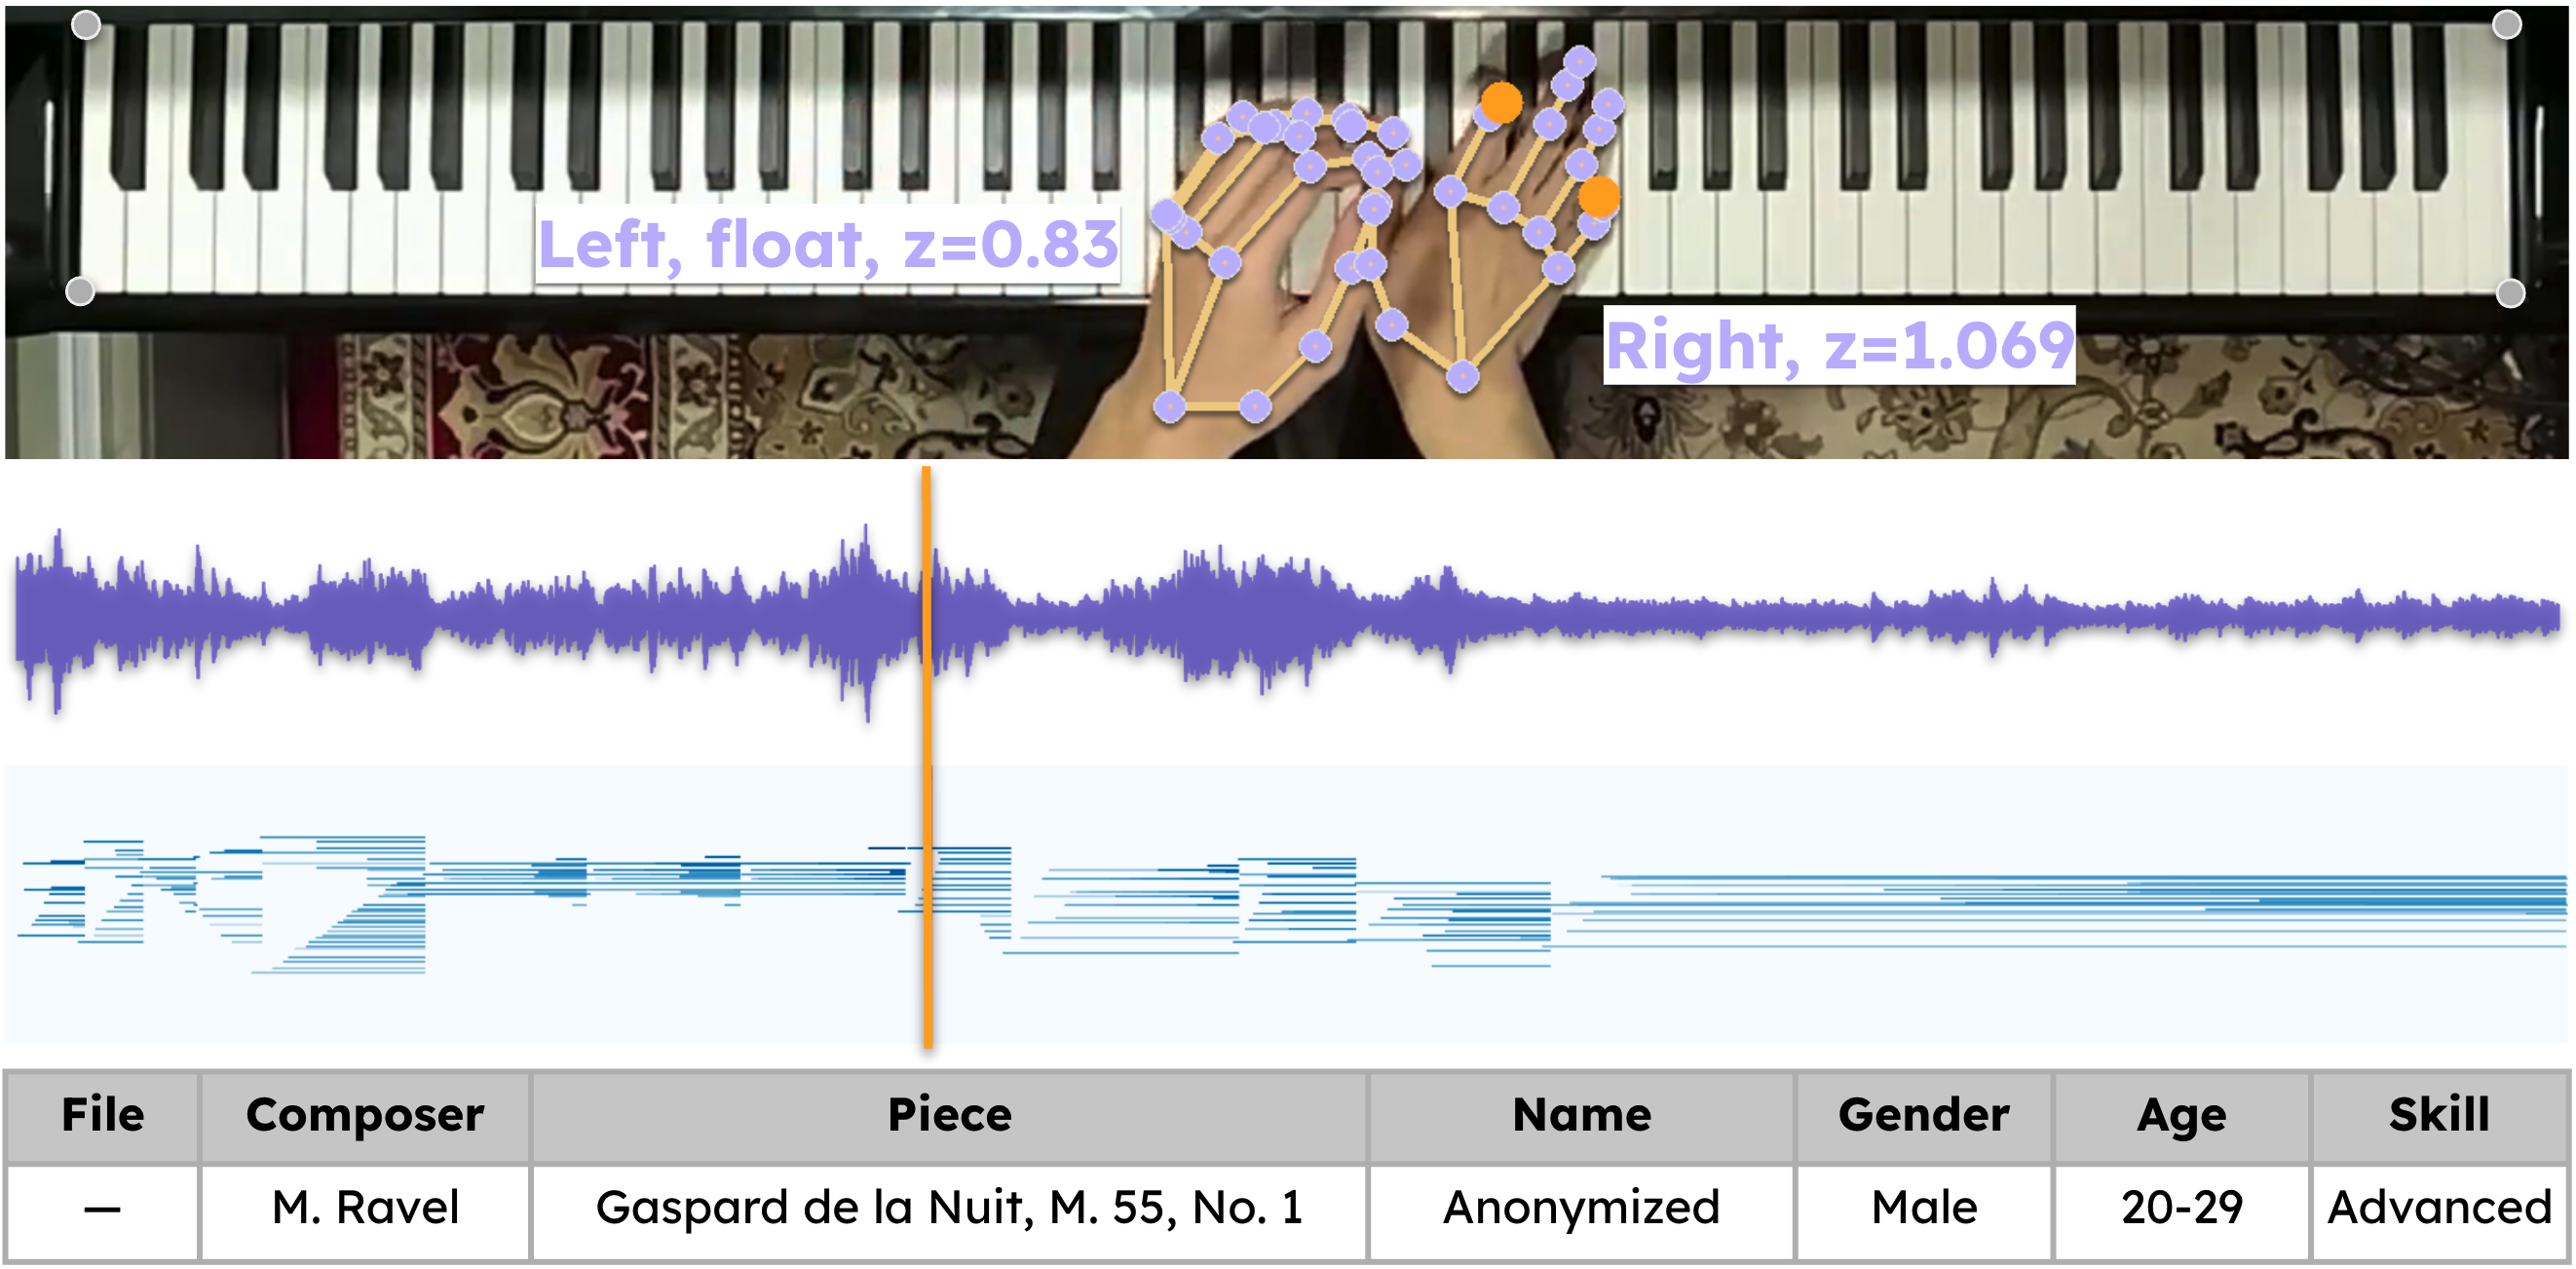
\includegraphics[width=1\linewidth]{Images/teaser_image.png}
    \caption{Overview of the PianoVAM dataset: A multimodal piano performance dataset featuring synchronized top-view video with keyboard coordinates, hand landmarks, fingering labels, audio, MIDI, and metadata.}
    \label{fig:enter-label}
\vspace{-5mm}    
\end{figure}

\section{Introduction}\label{sec:introduction}

%to enhance the extraction of musical information by leveraging multiple modalities \cite{IEEE19Duan, TMM18Li, MMSP20Montesinos, arXiv24Yoo, ICASSPW23Li}. 

Music performance is inherently multimodal, involving not only audio but also motion, posture, and other visual elements as part of the expressive sound creation process \cite{PPR09Bergeron, MusicPercep12Platz}. In the field of Music Information Retrieval (MIR), there has been growing interest in collecting multimodal performance data to enhance the extraction of musical information by leveraging multiple modalities \cite{TMM18Li, IEEE19Duan}. Such multimodal data ---particularly audio-visual data--- have been utilized in various MIR tasks across diverse musical genres. Examples include automatic MIDI transcription of solo piano performances \cite{ICASSP20Koepke, ICASSPW23Li}, vibrato analysis of polyphonic string music \cite{SMC17Li}, singing voice separation \cite{BMVC21Montesinos}, and melodic motif identification in Indian vocal performances \cite{TISMIR24Nadkarni}. In these tasks, visual information from performer videos has been shown to improve model robustness by providing additional musical cues. This paper focuses on the multimodal data collection of solo piano performances to improve transcription and explore other potential applications.  
%Music performance is inherently multimodal, extending beyond the auditory domain. Visual elements such as a musician's gestures, posture, and facial expressions can significantly contribute to the communication of musical intent and emotional expressivity \cite{PPR09Bergeron, MusicPercep12Platz}. These visual cues might play a critical role in audience perception and performance evaluation, sometimes even surpassing auditory information \cite{Moura2023, Tsay2013}. This underscores the importance of non-verbal expressivity in shaping how performances are perceived and appreciated.

% Beyond audience perception, it has been shown visual information can enhance key Music Information Retrieval (MIR) tasks \cite{IEEE19Duan, ISMIR24Choi}. In the context of piano performance, notable applications include Automatic Music Transcription (AMT) and fingering estimation. 

%Piano performance typically involves sheet music and performers. Sheet music contains not only musical notes to play but also directions to make the performing actions such as left-right hand split (indirectly from treble and bass staffs), fingering numbers, ...Performers provide information about musical expressions and fingering   
% diverse MIR tasks such as automatic music transcription, piano fingering, performer identification, performance 
% musical data such as audio, MIDI, fingering 


\begin{table*}[t]
    \centering
    \small
    \begin{tabular}{lcccccc}
        \toprule
        \textbf{Dataset}  & \textbf{Size (hrs)} & \textbf{Video} & \textbf{Audio} & \textbf{Audio Type} & \textbf{MIDI} & \textbf{Fingering} \\
        \midrule
        MAESTROv3 \cite{ICLR19Hawthorne}  & 198.7  & \xmark  & {44.1--48}\si{kHz}, Stereo & Real  & \cmark & \xmark \\
        MAPS (MUS subset) \cite{Emiya2010}     & 18.6  & \xmark     & 44.1\si{kHz}, Stereo & Synth. \& Real & \cmark & \xmark \\
        OMAPS2 \cite{ICASSPW23Li}   & 6.7  & 1080p/30fps & 44.1\si{kHz}, Mono & Real & $\triangle$ (.TXT)  & \xmark \\
        PianoYT \cite{ICASSP20Koepke}  & $\sim$20  & Varies  & Varies (YouTube) & Varies (YouTube) & $\triangle$ (Pseudo) & \xmark \\
%        PIAST \cite{NLP4MusA24Bang} & $\sim$1006 & \xmark & Varies (YouTube) & Varies (YouTube) & $\triangle$ (Pseudo) & \xmark \\
%        PianoMotion10M \cite{ICLR24Gan} & $\sim$116 & \xmark & 16\si{kHz}, Mono & Varies (Bilibili) & $\triangle$ (Pseudo) & \xmark \\
        PianoVAM (Ours) & 21.0 & 1080p/60fps & 44.1\si{kHz}, Mono & Real  & \cmark & $\triangle$ (Pseudo) \\
        \bottomrule
    \end{tabular}
\vspace{-2mm}    
    \label{tab:piano_datasets}
\caption{Comparison of piano transcription datasets.}
\end{table*}

\begin{table*}
    \centering

    \small
    \begin{tabular}{lcccccc}
        \toprule
        \textbf{Dataset}  & \textbf{Total notes} & \textbf{\# of pieces} & \textbf{Labeled ratio (\%)} & \textbf{Data type} & \textbf{Reliability} & \textbf{Annotation} \\
        \midrule
        PIG \cite{InfoSci20Nakamura} & 100,044 & 309 & 100 & MIDI \& Score & By pianists & Manual \\
        ThumbSet \cite{MM22Ramoneda} & -- & 2,523 & 52 & MusicXML & By miscellaneous & Manual \\
        PianoVAM-Finger (Ours) & 1,050,966 & 106 & 100 & Multimodal & $\sim$ 0.95 & Semi-Auto \\
        \bottomrule
    \end{tabular}
\vspace{-2mm}    
\caption{Comparison of Piano Fingering Datasets.}
    \label{tab:fingering-datasets}
\vspace{-2mm}    
\end{table*}

Piano transcription, which converts audio recordings into symbolic representations like MIDI or sheet music, is a well-established MIR task that has made significant progress through large-scale, clean audio-MIDI datasets such as MAESTRO \cite{ISMIR18Hawthorne} and carefully designed deep learning models \cite{TASLP21Kong, ISMIR22Wei}. As benchmarking performance on the MAESTRO dataset approaches its ceiling \cite{ISMIR24Yan}, new challenges have emerged in piano transcription. One major challenge is achieving acoustic robustness to ensure reliable transcription from real-world piano performance recordings, which often feature diverse piano timbres, reverberation, or other interfering noise sources. While data augmentation has been a common technique to address this issue \cite{ICLR19Hawthorne, Edwards2024}, leveraging visual data from performance videos has recently emerged as an alternative research direction \cite{CJE15Wan, DAFx21Wang, ICASSPW23Li, TASLP24Li}. Other key challenges include capturing richer performance information beyond a single MIDI track, such as left-right hand separation, piano fingering, and other playing details \cite{InfoSci20Nakamura, MM22Ramoneda}. Addressing these challenges requires capturing visual-domain data, such as performer motion or keyboard-view videos, and synchronizing them with audio and MIDI data. However, collecting such multi-modal data is costly, requiring a dedicated data acquisition system, and time-consuming, as it depends on the availability of prepared piano players. 

This paper introduces PianoVAM, a comprehensive piano performance dataset that includes videos, audio, MIDI, hand landmarks, fingering labels, and rich metadata. An overview of PianoVAM is presented in Figure \ref{fig:enter-label}. The dataset was collected from amateur pianists during their daily practice sessions on a Disklavier piano, with synchronized top-view videos captured in realistic and varied performance conditions. We extracted hand landmarks and generated fingering pseudo-labels using a pretrained hand pose estimation model combined with a semi-automated fingering detection algorithm.  We describe the challenges faced during data collection and the alignment of multiple modalities. Furthermore, we detail our fingering \alex{annotation} method, which utilizes hand landmarks extracted from the videos. Lastly, we present experimental results on both audio-only and audio-visual piano transcription using the PianoVAM dataset for benchmarking, along with a discussion of its potential applications.

%PianoVAM can be utilized in diverse research applications, including AMT, fingering estimation, performance analysis, performer identification and style analysis, and multimodal learning. This paper details the data collection and preprocessing procedures, presents an in-depth dataset analysis, and reports benchmark results for fingering detection and transcription. We evaluate how our dataset supports these tasks by comparing them with existing datasets and examining the added value of video data.

%audio-only transcription systems remain vulnerable in challenging acoustic conditions. To address the robustness issue, various data augmentation techniques have been explored \cite{ICLR19Hawthorne, Edwards2024}. Another direction  

% Although data augmentation techniques \cite{ISMIR24Kim, Edwards2024, ICLR19Hawthorne} have improved robustness, integrating visual data from performance videos has been shown to enhance onset prediction further \cite{CJE15Wan, DAFx21Wang, ICASSPW23Li, TASLP24Li}.

% AMT, which converts audio recordings into symbolic representations like MIDI or sheet music, has achieved significant progress through deep learning \cite{ISMIR18Hawthorne, TASLP21Kong, TASLP24Kwon}. However, audio-only transcription systems remain vulnerable in challenging acoustic conditions, such as noisy environments \cite{ISMIR24Kim}. While data augmentation techniques \cite{ISMIR24Kim, Edwards2024, ICLR19Hawthorne} have improved robustness, integrating visual data from performance videos has been shown to enhance onset prediction further \cite{CJE15Wan, DAFx21Wang, ICASSPW23Li, TASLP24Li}. Visual cues such as hand movements and keyboard interactions provide additional context that audio alone may not fully capture.


\section{Related Work}
% 데이터셋을 중심으로 최대한 작성해보려고 했습니다.
\subsection{Audio-Visual Datasets}
Audio-visual datasets have enabled or extended a range of MIR tasks by providing visual information complementing audio signals. The URMP dataset \cite{TMM18Li} offers synchronized audio, video, and MIDI recordings of multi-instrument classical performances, supporting multi-modal analysis of ensemble music such as audio-visual source association via vibrato modeling \cite{SMC17Li}. The Acappella dataset \cite{BMVC21Montesinos} contains solo a cappella videos, enabling audio-visual singing voice separation with fine-grained control over visual and acoustic conditions. Nadkarni et al.\ present an audio-visual dataset of Hindustani vocal performances annotated with melodic motifs and stable notes, enabling gesture-based music analysis and raga classification through movement-melody correspondence \cite{TISMIR24Nadkarni}.

% Among multimodal formats, audio-visual data have been influential, as synchronized visual data can provide complementary information, which may be challenging to extract from audio alone.

% demonstrated that fine-grained vibrato motion captured from performer videos can be effectively correlated with pitch fluctuations in polyphonic string music, enabling accurate audio-visual source association in ensemble performances.

%Existing piano performance datasets typically address isolated or limited modalities (see Table \ref{tab:piano_datasets}). For instance, 

\subsection{Piano Transcription Datasets}
Table~\ref{tab:piano_datasets} compares existing piano performance datasets with PianoVAM. MAESTRO \cite{ICLR19Hawthorne} includes high-quality audio and MIDI data recorded from proficient pianists on Disklavier pianos but lacks top-view videos. While MAPS \cite{Emiya2010} provides audio and MIDI from actual performances (MUS subset), a significant portion (210 out of 270 recordings) is synthesized. OMAPS2 \cite{ICASSPW23Li} and PianoYT \cite{ICASSP20Koepke} incorporate video data but offer only limited MIDI annotations: OMAPS2 provides MIDI-like labels, while PianoYT uses pseudo-MIDI annotations transcribed with the Onsets and Frames model \cite{ISMIR18Hawthorne}. In comparison, PianoVAM offers the most comprehensive multi-modal dataset, including real performance audio, synchronized MIDI, top-view videos, and fingering pseudo-labels, although its total duration is limited compared to the larger datasets listed.

% PIAST \cite{NLP4MusA24Bang} provides extensive audio data and metadata but rely on pseudo-MIDI annotations. PianoMotion10M\cite{ICLR24Gan}  provides 116 hours of bird’s-eye-view video with audio and over 10 million annotated hand poses, focusing primarily on hand motion and fingering guidance rather than note-level transcription. \jh{how about removing PianoMotion10M if it is not for transcription?}

%\jh{add a description of PianoMotion10M here}

%transcribed via \cite{TASLP21Kong} and lack video content. 


\subsection{Fingering Datasets}
% 기존에 존재하는 데이터셋을 소개하는 느낌으로 작성을 해야할 것 같아요. 글을 Table 2와 함께 볼 수 있도록!

Table \ref{tab:fingering-datasets} compares existing piano fingering datasets with PianoVAM. PIG \cite{InfoSci20Nakamura} incorporates fingering and MIDI information of sections of several pieces played by professional pianists, which also provides different fingerings for the same piece by various pianists. Ramoneda et al.\ \cite{MM22Ramoneda} tried to annotate fingering of the complete piece from partially annotated MusicXML files with the support of ThumbSet dataset, which in turn crowd-sourced fingering information of numerous pieces from MuseScore\footnote{\href{https://musescore.com}{https://musescore.com}, \alex{add access date}}, an online piano score website, but the source of fingering annotation is not clear. The presented PianoVAM-Finger dataset, in contrast, utilizes a fingering detection algorithm  applied to top video data synced with MIDI and is improved by manual annotation of incomplete fingering labels to improve reliability.  

% While not only achieving large-scale coverage with over one million meticulously labeled notes, PianoVAM-Finger but also integrates high-resolution video, audio, and MIDI in a genuinely synchronized manner, providing an extensible resource that can substantially advance research on fingering estimation, performance analysis, and multimodal MIR applications.

%저는 이렇게 정리해봤는데, 참고하셔요. - 준형  감사합니다!! - 준형 (small) 이게 더 나은것 같은데요 ㅋㅋ ㅋㅋㅋ 쓸모있다면 ㄱㄱ

%Consequently, PianoVAM-Finger not only achieves large-scale coverage with over one million meticulously labeled notes but also integrates high-resolution video, audio, and MIDI in a genuinely synchronized manner, providing an extensible resource that can substantially advance research on fingering estimation, performance analysis, and multimodal MIR applications.

%\jh{add some sentences that explains the strength of our dataset}

% In piano performance, fingering data is recognized as a key factor directly linked to technical proficiency and expressive interpretation \cite{Piano21Telles}. Data-driven methods are major trend in the field of fingering estimation, however they primarily rely on audio and symbolic data \cite{IEAAIE10Maezawa, InfoSci20Nakamura, MM22Ramoneda}, yet they can yield inconsistent results due to the variability of the training data. In contrast, performance video provides direct visual information on finger placement and movement, enabling more reliable analyses \cite{MM07Zhang}. 

% As summarized in Table \ref{tab:fingering-datasets}, this lack of 

% PIG\cite{IEAAIE10Maezawa} dataset은 Pianist들이 직접 musical piece들의 section을 annotating 했으며, 같은 section에 대해서 여러 명의 pianist가 서로 다른 fingering을 labeling 하기도 하였다. \cite{MM22Ramoneda} tried to annotate fingering from partially annotated scores via ThumbSet: this dataset은 MuseScore\footnote{https://musescore.com}에 musicXML 정보와 함께 제공되어 있는 fingering information (source is not clear라고 언급되어있음) 를 사용해서 fingering 정보를 crowdsource 하였지만 MIDI 정보는 제공되지 않음. Discussion에 우리 dataset은 전체 곡을 clear하게 연주하지 않고, 연주자가 편하게 연습하듯이 일정 부분을 반복한다던가 mistouch가 있다는 점도 적어야 할듯!!

% PIG \cite{IEAAIE10Maezawa} incorporates fingering annotation of sections of several pieces played by professional pianists, which also provides different fingerings for the same piece by various pianists. In \cite{MM22Ramoneda}, they tried to annotate fingering from partially annotated scores with the support of ThumbSet: which crowdsourced fingering information of numerous pieces from MuseScore\footnote{https://musescore.com}, the online piano score website, but the source of fingering annotation is not clear.


% However, the shortage of synchronized datasets that integrate audio, video, symbolic notation, and explicit fingering annotations has hindered active research into video-based fingering detection based on these data.
 


% To address these limitations, we introduce \textbf{PianoVAM}, a comprehensive 21-hour Video-Audio-MIDI dataset designed explicitly to support diverse applications in piano performance. PianoVAM features synchronized top-view performance videos, audio, MIDI data, and fingering labels obtained via our suggested rule-based algorithm based on MediaPipe and complemented by human annotations, extracted hand landmarks, and rich metadata.


%score-following and accompaniment systems, performance analysis, performer identification and style analysis, and multimodal learning and music generation. We briefly list these areas here and elaborate further in Section \ref{sec:fingering_detection}, \ref{sec:transcription} and \ref{sec:future-rsearch-directions}.


% This paper details the data collection and preprocessing procedures, presents an in-depth dataset analysis, and presents benchmark results for fingering detection and transcription. We compare its performance against established datasets and investigate the benefits of incorporating video data. 
% By publicly releasing PianoVAM, we aim to encourage research at the intersection of piano performance, machine learning, and multimodal signal processing.

\section{Dataset Acquisition \& Pre-processing}\label{sec:dataset-acquisition-preprocessing}
PianoVAM is available for download from the GitHub website\footnote{https://yonghyunk1m.github.io/PianoVAM\label{github-link}\alex{add href and access date}} or Hugging Face.\footnote{anonymized huggingface link\alex{add link and access date}} A small subset of the dataset and data loader are also provided for convenience.

\subsection{Acquisition}
%Acquiring synchronized piano performance video, audio, and MIDI is challenging, particularly in achieving precise alignment across modalities. Efficient metadata collection, such as piece details and performer information, is best integrated into the acquisition process but should remain unobtrusive to both performers and annotators. To address these challenges, we developed PiaRec, a dedicated system designed to optimize user experience and streamline data collection. PiaRec enables performers to contribute data independently, without external assistance, while automating post-processing to achieve approximate synchronization between audio and video, minimizing manual effort.

We developed a data acquisition system that enables performers to record video, audio, and MIDI independently with minimal manual effort, while seamlessly integrating unobtrusive metadata collection, such as piece details and performer information.  
 
% Collecting synchronized piano performance video, audio, and MIDI is challenging, especially when aiming for precise alignment. Our dedicated data-collection system addresses this by enabling performers to record independently and automating essential synchronization. The system also integrates unobtrusive metadata collection, such as piece details and performer information.
% \figref{fig:piarec} visualizes some aspects of the acquisition setup.

%\begin{figure}
%    \centering
%    \includegraphics[width=\linewidth]{Images/PiaRec.png}\hspace*{0cm}
%    \caption{Recording environment and setup.}
%    \label{fig:piarec}
% \end{figure}

%\textbf{User Registration:} First-time users must complete a registration process that collects key performer information, including self-assessed proficiency (categorized into three levels: Beginner, Intermediate, Advanced), age group, and gender. Upon successful registration, users receive an email containing three QR codes: one associated with their profile and two for system control, serving as triggers to start and stop recording. 

%\textbf{System Initialization:} The recording environment is activated by clicking the PiaRec launch button, integrated with StreamDeck for convenience. This action initializes the PiaRec main interface, OBS Studio for video and audio recording, and Logic Pro for audio and MIDI recording, all displayed on the PC screen.

%\textbf{Recording Setup:} Before each session, users enter performance-specific details in the Record tab. All required fields must be completed before proceeding.

%\textbf{Recording Process:} After confirming performance details, users display their profile QR code to the top-view camera. PiaRec then activates the previously initialized recording software (OBS Studio and Logic Pro).

%\textbf{Stopping the Recording:} During the performance, the system continuously monitors for QR code events. Displaying the stop QR code prompts PiaRec to halt all recordings. PiaRec then aligns the tracks by comparing the first 10 seconds of each recorded audio file, trimming the earlier track to ensure proper synchronization. (See Section \ref{subsubsec:alignment} for detailed synchronization procedures.)

\begin{figure*}
    \centering
    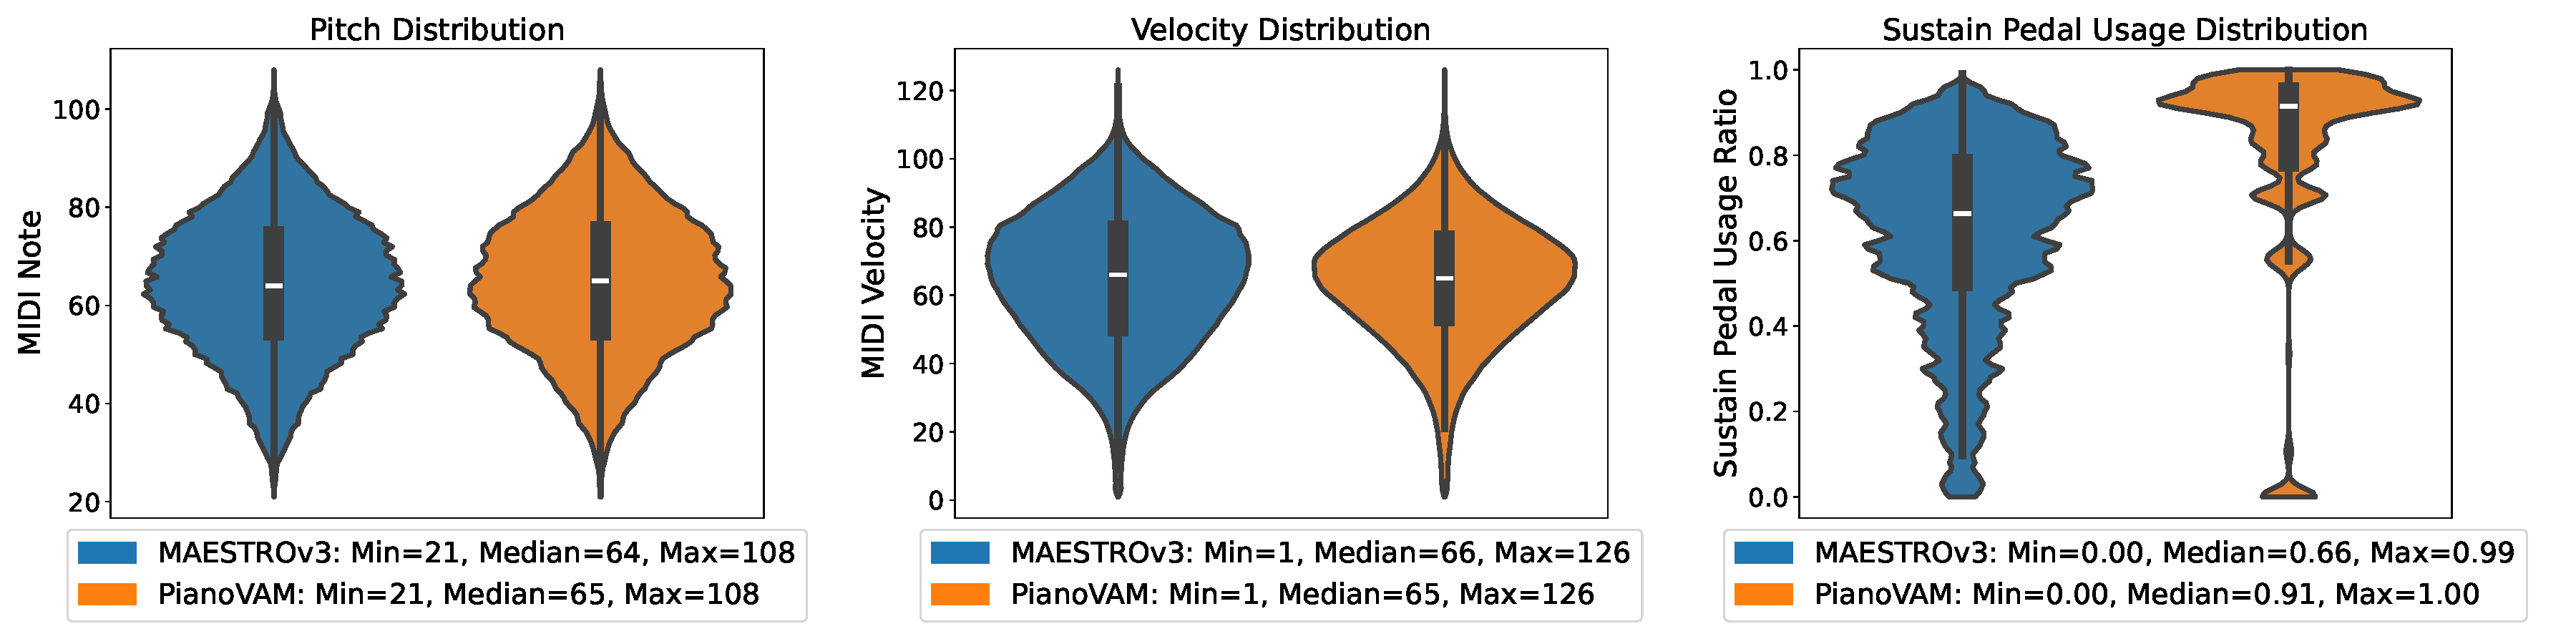
\includegraphics[width=1\linewidth]{Images/combined_violinplot.pdf}
    \vspace{-7mm}    
    \caption{Distributional comparison of pitch, velocity, and pedal usage between MAESTROv3 and PianoVAM.}
    \label{fig:combined-violinplot}
\end{figure*}


\subsubsection{Acquisition Workflow}
The acquisition workflow comprises the following steps. 
%A dedicated data-collection process allows performers to record piano performances with minimal manual effort. 
First, new users register by providing basic personal details and receive unique QR codes for identification and recording control. A single interface launch initializes the required software: OBS Studio for video and audio, and Logic Pro for audio and MIDI. Before recording, users input performance details and display their profile QR code to a top-view camera to begin capturing. When the performance concludes, presenting a stop QR code ends the recording. % The system cross-correlates the initial seconds of audio tracks to synchronize video, audio, and MIDI.


\subsubsection{Hardware Setup} 
A PC runs the control script along with OBS Studio and Logic Pro. A webcam mounted overhead provides the video feed, and a microphone records audio. Logic Pro captures the MIDI output of the Disklavier piano. Recording the same audio source in OBS Studio and Logic Pro enables approximate synchronization between video and MIDI.

\subsection{Pre-processing}
\subsubsection{Alignment}\label{subsubsec:alignment}
%https://docs.google.com/document/d/1G1aIxIEiFI9kxwOgP_GDq4pADkeToc136394PAb-5-I/edit?usp=sharing

The time alignment of audio and MIDI data was further refined using the fine alignment technique used for the MAESTRO dataset \cite{ICLR19Hawthorne}.
% While the MAESTRO approach employs coarse and fine alignment steps to mitigate large misalignment and residual jitter, only the fine alignment procedure was adopted here because no substantial misalignment was observed. 
Specifically, the recorded audio was down-mixed to mono and resampled to {22.05}\si{kHz}. 
The MIDI data was then synthesized into an audio signal at the same sampling rate using FluidSynth with a SoundFont sampled from Disklavier Pro recordings,\footnote{\href{https://freepats.zenvoid.org/Piano/YDP-GrandPiano/YDP-GrandPiano-SF2-20160804.tar.bz2}{https://freepats.zenvoid.org/Piano/YDP-GrandPiano/YDP-GrandPiano-SF2-20160804.tar.bz2} (Last accessed: March 28, 2025)\label{soundfont}} 
\alex{necessary?: since we could not access the original Disklavier7 SoundFont path used in the MAESTRO dataset}.
A Constant-Q Transform was applied to both audio signals using a hop length of 64 samples ($\sim$3\si{ms} resolution). Finally, we applied Dynamic Time Warping within a Sakoe-Chiba band of $\pm2.5$\si{s} to detect and correct any remaining temporal discrepancies, such as small constant offsets or jitter.


\subsubsection{Audio Loudness Normalization}
% While piano transcription models are generally designed to predict MIDI velocity independently of the absolute audio loudness, ensuring a consistent correspondence between MIDI velocity values and loudness of audio samples in the dataset should be maintained not to confuse models during training \cite{}.  
Recordings were collected over a six-month period in a shared studio, with a notable gap between May and August. This interruption may have introduced inconsistencies in loudness due to variations in recording conditions, such as gain settings or microphone placement. To mitigate potential mismatches between loudness and MIDI velocity across the dataset, we applied a loudness normalization procedure. First, the collected MIDI data were synthesized using \textit{FluidSynth} with a Disklavier-sampled SoundFont.\footref{soundfont} The integrated loudness of each synthesized audio file was measured using the \textit{pyloudnorm} package. We then computed the average loudness across all rendered files and defined $-$23~\si{LUFS} as the desired global average. A uniform gain offset was calculated based on the difference between the measured average and this target. This offset was added to each file's measured loudness, resulting in a new target loudness for normalization. Each real PianoVAM audio recording was then normalized to match its corresponding target.\alex{this is still not clear. 'target' above refers to -23LUFS, but it seems target changes its meaning during the description? It might be clearer if you said something like: Each real PianoVAM audio recording was then normalized to match the loudness of its synthesized counterpart. The average loudness of the dataset was subsequently adjusted to -23 LUFS.} This process is designed to enhance loudness-velocity consistency while preserving the natural dynamic range of the performances.

% The loudness of each rendered audio file was then measured using the \textit{pyloudnorm} package.

% We will not include this Figure.
%\begin{figure}
 %   \centering
  %  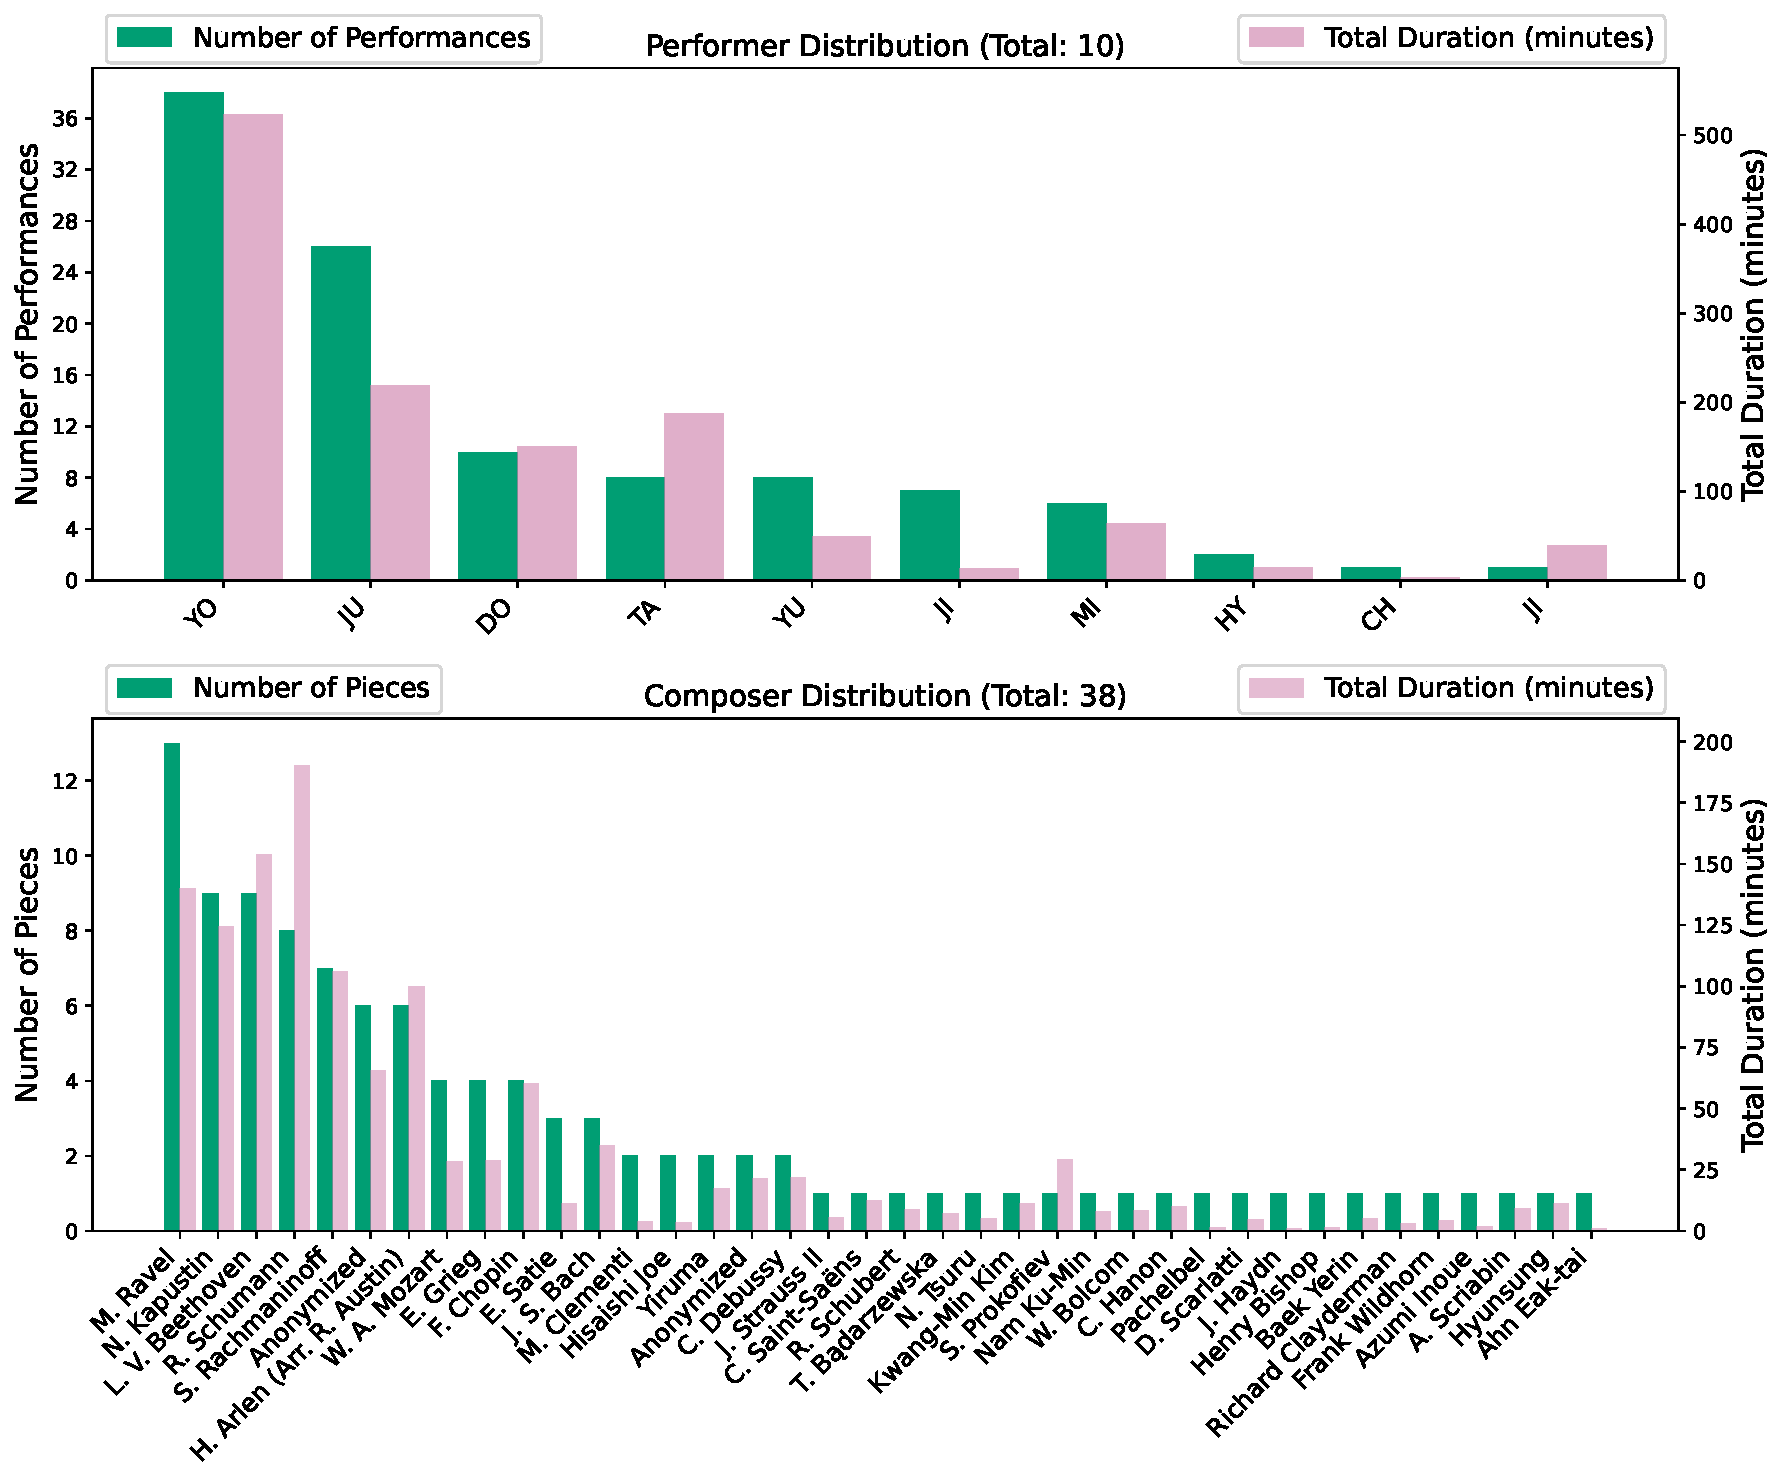
\includegraphics[width=\linewidth]{Images/performer_composer_distribution.pdf}\hspace*{0cm}
  %  \caption{Performer and composer distribution.}
   % \label{fig:performer_composer_distribution}
%\end{figure}

\section{Dataset Statistics}\label{sec:dataset-statistics}

The dataset comprises 106 recordings spanning approximately 21 hours, featuring 10 unique amateur performers and 38 composers. The included repertoire covers Baroque through modern works, featuring composers such as Bach, Chopin, Schumann, Kapustin, and Joe Hisaishi, alongside several improvisations. This range illustrates the dataset's focus on a broad scope of historical periods and performance practices. All recordings are solo performances. Self-reported skill levels include 70 advanced, 26 intermediate, and 10 beginner-level recordings. Although the recording system allowed performers to choose between two performance types ---Performance and DailyPractice--- all recordings were self-labeled as DailyPractice. This indicates that the dataset primarily captures informal, practice-oriented sessions, which may deviate from the strict adherence to score information typically expected in formal stage performances. 

To investigate differences in expressive characteristics across datasets, we conducted a brief comparative analysis of MIDI-related distributions between MAESTROv3 and PianoVAM. Specifically, we examined three aspects displayed in \figref{fig:combined-violinplot}: 
\begin{inparaenum}[(i)]
    \item the distribution of pitch (MIDI note numbers), 
    \item the distribution of velocity (MIDI velocity values), and 
    \item the distribution of sustain pedal usage on a per-file basis.
\end{inparaenum}
We computed Cohen's \textit{d} for each musical feature to assess the practical significance of inter-dataset differences.  Pitch (\textit{d} = 0.0446) and velocity (\textit{d} = -0.0379) exhibited negligible differences between datasets. However, pedal usage revealed a large effect size (\textit{d} = 0.870), indicating a substantially higher use of the sustain pedal in PianoVAM compared to MAESTROv3. 
 

%이는 곡 레퍼토리적 이유와 실제 연주 환경 양측이 모두 영향을 준 것으로 추정할 수 있습니다. 먼저, 연주된 곡에서 낭만주의·인상주의 작품군이 많다는 점}에서 음색의 풍부함과 긴 레가토 표현을 위해 페달을 빈번히 사용하게 되고, 실제 곡 난이도나 음역이 넓은 협주곡·판타지 등이 많다는 점 또한 페달 의존도를 높이는 원인이 됩니다. 동시에 아마추어 연주자들이 연습 과정을 녹음했다는 상황적 특성도 작용할 수 있는데, 곡 해석이나 테크닉 측면에서 페달을 좀 더 “길게” 혹은 “자주” 밟아 울림을 유지하려는 경향, 나아가 녹음 환경에서 음색을 풍부하게 만들려는 ‘과다한 페달링’이 발생할 여지가 크기 때문입니다.

% 페달의 사용이 음원에서의 울림정도와 관련이 있지만, 레코딩 환경 역시 중요. Blind RT60\cite{ICASSP14Dumortier}에서 제공하는 RT60을 각 데이터별로 분석을 해보았다. (The RT60 is defined as the time required for sound to decay by 60 dB once the source has been switched off.)
% % (Mar 26 22:13; Ongoing for Getting the Result)
% 일단 preliminary result로는 MAESTRO가 실제 concert hall에서 녹취된 음원이어서 Studio에서 녹취된 우리 데이터셋보다 울림이 크다. 

\section{Annotation of Fingering Labels}\label{sec:fingering_detection}
This section presents a semi-automated fingering annotation algorithm. 
%As the collected data includes both video and audio, the dataset can also be helpful for other tasks beyond transcription. One example is visual fingering analysis. Utilizing MediaPipe Hands~\cite{arXiv20Zhang}, a widely-used hand landmark detection framework, we created fingering annotations in a semi-automated way.
The processing pipeline of this algorithm is visualized in \figref{fig:fingering_diagram}: it extracts skeletal hand coordinates from performance videos and maps them to the corresponding MIDI notes, achieving a precision of approx.\ 95\%. However, the algorithm missed approx.\ 20\% of MIDI notes showing difficulties in handling complex playing techniques and ambiguous finger positions in videos. To address these gaps, we developed an efficient GUI-based fingering annotation tool, allowing human annotators to supplement missing fingering labels. By combining the results of the automated algorithm with manual additions and corrections, complete fingering annotations for all MIDI notes in the PianoVAM dataset can be provided.

\subsection{Inputs \& Outputs}
The inputs are video, MIDI, keyboard corner locations and lens distortion coefficients in the first frame for each video, which can also be set manually by the GUI-based annotation tool.
%Note that the input data needs a few pre-processing to apply our algorithm to other multimodal datasets.
The outputs are fingering information, and a separate MIDI file  for each hand.

%아니면 다른 데이터셋에서도 활용할 수 있rmfjf t다는 걸 강조하기 위해서 그냥 video and midi synced in 5ms 정도로만 적어도 괜찮을까 싶네요. (Junhyung)



\subsection{Method}
% 
\begin{figure}
    \centering
    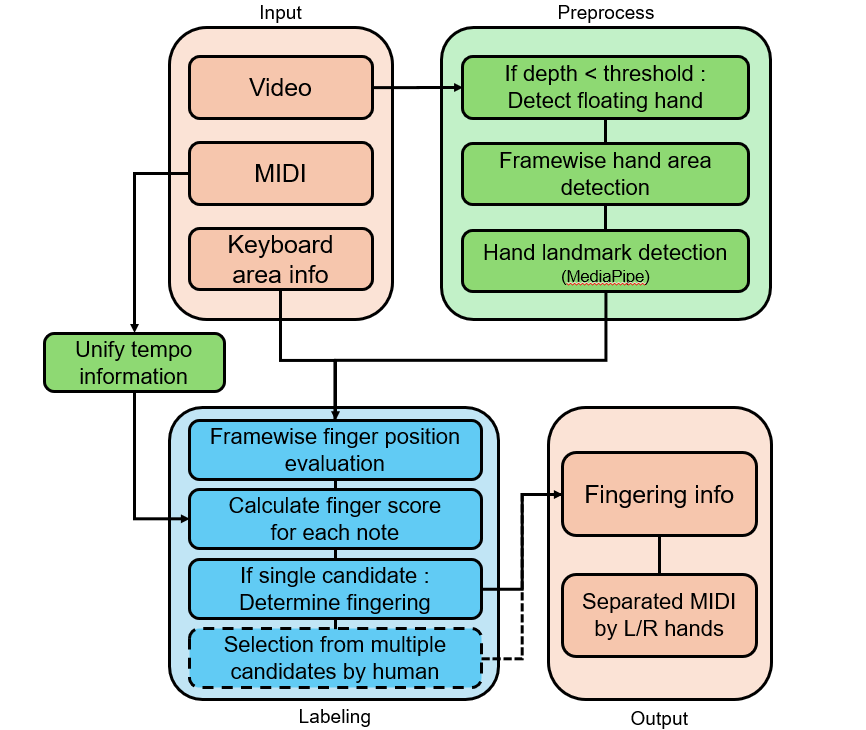
\includegraphics[width=\linewidth]{Images/fingering_detection.png}\hspace*{0cm}
    \caption{Process diagram of the fingering detection algorithm.}
    \label{fig:fingering_diagram}
\end{figure}

The algorithm suggests candidates of fingers that are likely to play each note in the MIDI file. First, hand landmark information is extracted from the input video frame with MediaPipe Hands~\cite{arXiv20Zhang}. A floating hand obfuscating the other hand but not playing any notes should be detected and be excluded from the candidates. Thus, we define a metric to measure the $z$-depth of a hand to detect floating hands. Assuming that we know the hand skeleton of the player explicitly, we can calculate the $z$-depth from the $xy$ coordinate information. For each video, we find the \textit{model skeleton} of each hand, which is a standard for all skeletons that should be unbent, not tilted, and on the keyboard. To measure tilt, the plane defined by three hand key points, namely Wrist ($W$), Index Finger Metacarpals ($I$), and Ring Finger Metacarpals ($R$), is utilized. We assume that the angle $\angle IWR$ of the untilted skeleton (parallel to the plane of the keyboard) should be close to $28\degree$, which is our heuristic estimate for the average human hand in its neutral position. To measure how much the hand is bent, we calculate the ratio $r=\frac{|\triangle IWR|}{|WF_{1}F_{2}F_{3}F_{4}F_{5}|}$ of $|\triangle IWR|$ and area of the hexagon $|WF_{1}F_{2}F_{3}F_{4}F_{5}|$ where $F_i$ is the fingertip of the $i$th finger. Finally, assuming that the hand is playing in the majority of frames, the median $\triangle IWR$ is selected as the default position:
\begin{equation}
    I_{0}W_{0}R_{0}=\underset{|\angle IWR - 28\degree| \text{ low 10\%}, r \text{ high 50\%}}{\text{median}}|\triangle IWR| .
\end{equation}
Let the plane of the projected 2D image be $z=z_{0}$, and the area of 2D image be
\begin{equation}
  \begin{aligned}
    A:=\{(x,y)  | x\in (-1,1), y\in (-AR,AR)\} \subset \mathbb{R}^2
    \\\cong\{(x,y,z_{0})|x\in(-1,1), y\in (-AR,AR)\}\subset \mathbf{P}\mathbb{R}^3 ,
\end{aligned}  
\end{equation}
where the origin of real projective space $\mathbf{P}\mathbb{R}^3$ is the center of the lens of the camera and $AR$ is the aspect ratio of the video. Since the goal is to calculate the relative depth rather than the real depth, we set $z_{0}=1$ for convenience of calculation.
%Now we are ready to calculate the relative $z$-depth of the hands. 
Knowing that the original point is contained in the line $\{(xt,yt,t) | t\in \mathbb{R^{+}}\}$, we have three equations likely in general position and three variables to solve $t,u,v>0$ from
\begin{gather}
    \left||(x_{I}t,y_{I}t,t),(x_{W}u,y_{W}u,u)|\right|_{\mathbb{R}^3}=\left|\overline{I_{0}W_{0}}\right| \\
    \left||(x_{W}u,y_{W}u,u),(x_{R}v,y_{R}v,v)|\right|_{\mathbb{R}^3}=\left|\overline{W_{0}R_{0}}\right| \\
    \left||(x_{R}v,y_{R}v,v),(x_{I}t,y_{I}t,t)|\right|_{\mathbb{R}^3}=\left|\overline{R_{0}I_{0}}\right|.
\end{gather}
%
Our desired solution can be approximately calculated using Powell's dog leg algorithm with a close initial guess $(t_i,u_i,v_i)=(1,1,1)$. By substituting the solution $(t,u,v)$, we get the 3D coordinates of $I,W,R$.  Finally, $d=(t+u+v)/3$ becomes the relative $z$-depth of the mass of the center of the hand skeleton of each frame. If the $z$-depth is less than the threshold $0.9$, or equivalently, if the hand is floating more than 10\% of the distance between the camera and the keyboard, we decide that the target hand of the target frame is floating.

% Note that if three elliptical cylinders are in general position, there must exist a solution. Also, the number of solutions is at most 4 by B\'{e}zout's theorem and symmetry. Here, our desired solution can be approximately calculated using Powell's dog leg algorithm with a close initial guess $(t,u,v)=(1,1,1)$.
% Finally, $d=\displaystyle\frac{t+u+v}{3}$ becomes the $z$-depth of mass of the center of the hand skeleton of each frame. From (3)$\sim$(5), it is obvious that $d_{\text{model}}=1$ for each hand.\\
% Now, we decide that the targeted hand of targeted frame is floating if (6) holds: 
% \begin{equation}
%     \frac{1}{2}\mathbf{d}_{\pm k\text{frames}} \cdot \frac{1}{k(k-2)}[1,2,\cdots, k,\cdots, 1]+\frac{1}{2}d_{\text{frame}}<0.9
% \end{equation} where $\mathbf{d}_{\pm kframes}$ is vector of depths of $2k-1$ frames near the target frame, and if there are some frames unavailable to detect targeted hand with MediaPipe, instead we just use depth of the targeted frame. In (6), we consider the depth of close frames as hand motion is continuous. Empirically, we involved 0.25 seconds of finger motion to the finger score, in other words, $k=7$.\\

% \begin{algorithm}[h]
% \caption{Fingering Candidate Selection Algorithm}\label{alg:cap}
% \begin{algorithmic}
% \State $N = \text{Total number of notes}$
% \State $K(n) = \text{Keyboard area of $n$th note}$
% \State $R(n) = \text{Range of frames of $n$th note played}$
% \State $H(f,i) = i\text{th Finger location info of frame $f$,} $ but fingers of floating hands are not contained
% \State $w = \text{width of a key}$ 
% \For{$n < N$}
% \State $S_n \gets (0,0,\cdots, 0)$ \Comment{Score of each finger likely playing $n$th note}
% \For{$f \in R(n)$}
% \For{$i<10$}
% \If{\text{each }$H(f,i) \in K(n)$}
% \State $S_n\gets S_n + \chi_i$ \Comment{$\chi_i$ = $i$th unit vector}
% \ElsIf{$0<||H(f,i),K(n)||_{\mathbb{R}^2}< w$}
% \State $S_n \gets S_n + \left(\frac{1-||H(f,i),K(n)||_{\mathbb{R}^2}}{w}\right)^{2}$
% \EndIf
% \EndFor
% \EndFor
% \EndFor
% \For{$n<N$}
% \If{$\exists i \ s.t. \ S_n \cdot \chi_i > 0.5|R(n)|$}
% \If{$\exists ! \ i$}
% \State $i$ is the only candidate
% \ElsIf{$\exists ! \ i \ s.t. \ S_n \cdot \chi_i > 0.8|R(n)|$}
% \State $i$ is the only candidate
% \Else \text{ }  There are multiple candidates
% \EndIf
% \Else \text{ } There are no candidates
% \EndIf
% \EndFor
% \end{algorithmic}
% \end{algorithm}

After discarding all floating hands from the detection, possible finger candidates for each note can be chosen. For each note, a fingering score is calculated, indicating the likelihood of each finger pressing the note. The score is based on the number of frames in which the fingertip is in the selected note area. If the fingertip is completely in the area, a value of 1 is assigned; if it is slightly off, a correction weight is applied, reducing the score for this frame. Thus, the final fingering score cannot exceed the total number of frames of each note.\\
From the fingering score of each finger for the $n$th note, we add the finger as a normal candidate or a strong candidate if the fingering score is greater than 50\% or 80\% of the theoretical maximum score (note length in frames), respectively. If there exists only one strong candidate, we pick the strong candidate as the only candidate. Note that there might be notes with either no candidate or multiple candidates, in which case the algorithm will leave these notes unlabeled.

\subsubsection{Reliability}
With the support of the dedicated GUI-based fingering annotation tool, we manually labeled the ground truth fingering for the first 150 notes of 10 pieces in PianoVAM to assess the results. Table \ref{tab:fingering_results} shows the precision of our fingering algorithm for the first 150 notes of 10 pieces in PianoVAM. The average precision exceeded 95\%, with most false fingerings involving adjacent fingers to the ground truth. The table also reports the percentage of notes with no candidates and multiple candidates. %The weighted averages are 9.4\% and 5.2\%. 
An outlier is Ravel's \textit{Jeux d'eau} with a very high ratio of notes without candidates; the weighted averages excluding \textit{Jeux d'eau} were 9.4\% and 5.2\%.

\begin{table}
\def\sym#1{\ifmmode^{#1}\else\(^{#1}\)\fi}
\centering
\small

\begin{center}
\begin{tabular*}{\columnwidth}{l@{\extracolsep{\fill}}ccc}
%\begin{tabular}{l c c c}
\toprule
\multirow{2}{*}{\textbf{Piece (Index)}} &  \textbf{Prec.} & \textbf{Total}  & \textbf{Total} \\                                     &  \textbf{(150)} & \textbf{No C.} & \textbf{Multi C.}\\
\midrule
Chopin, Op.18 (8) &  91.7 & 12.7 & 8.0 \\
Debussy, L.75 Mvt.3 (17)\sym{*} & 97.1 & 7.9 & 2.8 \\
Grieg, Op.16 Mvt.2 (18) & 99.3 & 10.6 & 4.4 \\
Yiruma, Kiss the Rain (29) & 95.2 & 5.9 & 8.7 \\
Improvisation (31) & 98.6 & 16.7 & 3.0 \\
Schumann, Op.17 Mvt.1 (34) & 82.9 & 8.0 & 5.4 \\
Kapustin, Op.40 No.6 (42) & 98.4 & 8.4 & 5.5 \\
Scarlatti, K.380 (60) & 100.0 & 3.7 & 3.5 \\
Ravel, M.30 (81) & 92.4 & 35.1 & 4.4 \\
Satie, Gymnopedie No.1 (93) & 100.0 & 4.1 & 2.4 \\ 
\midrule
\textbf{Average of 10 pieces} & 95.6 & 13.0$^\dagger$ & 5.1$^\dagger$
\\
% \textbf{Total 107 pieces} & $-$ & & \\
\bottomrule
\end{tabular*}
\caption{Precision (\textit{Prec.}) over first 150 notes, percentage of notes with none or multiple candidates (\textit{C.}) over all notes for selected 10 pieces (\sym{*}For finger substitutions, we admit both fingers as correct fingering. $^\dagger$Weighted average with the number of total notes of each piece as the weight.)}
\label{tab:fingering_results}
\end{center}
\end{table}
% Compared to other fingering datasets such as PIG\cite{InfoSci20Nakamura} and ThumbSet\cite{ACM22Ramoneda}, our algorithm provides the opportunity to make a large-scale fingering dataset by applying our algorithm to other datasets that have MIDI data synced with top-view videos. In particular, we expect high-quality fingering from datasets with more advanced performers. \\ 
%\\ %Chopin's waltz contains fast note repetition, which makes several fingers above the note to prepare to play that repeated note. In this situation, our algorithm will make false decisions since several fingers are in the note area and in full note length, since the note length is very short, in the range of about 2 or 3 frames. Also, MediaPipe can mispredict fingertip keypoints under shadow, which is the main reason for false decisions of Schubert's fantasie data. Otherwise, blurry frame images, head interruption, or sleeve interruption can affect the misprediction of MediaPipe and our algorithm. We expect that using newer hand pose estimation models such as ViTPose+ \cite{} can lead to higher precision.
% Moved to discussion

%PIG dataset, ThumbSet dataset 비교
%Hyperparameter justification 

% \section{Benchmark Results}\label{sec:transcription}
% % Automatic Music Transcription (AMT) is a key research area in Music Information Retrieval (MIR), particularly for piano transcription. While AMT systems have traditionally relied on audio as the primary input, some recent studies have explored the use of video data.
% Koepke et al.~\cite{Koepke} introduced Visual Music Transcription (VMT), which leverages video to predict note onsets. Other approaches \cite{,} incorporate visual information in post-processing to refine onset predictions in audio-only AMT systems. Additionally, a two-stage method trains audio and video modules separately and then fuses their features for onset prediction. These efforts highlight the potential of visual data in music analysis.

\section{Benchmark Results}\label{sec:transcription}

% Data Split

% A unique 4-hands performance (2024-02-15\_22-12-41) was assigned to the special split, as it may present a special case for deep learning models that incorporate video inputs.

We assess the transcription of the dataset for benchmarking in two piano transcription settings: audio-only and audio-visual. In the audio-visual setting, we specifically examine the visual modality's contribution to enhancing acoustic robustness. 
% These modalities reflect current trends in the field and underscore the dataset's potential as a useful resource for both tasks.

\subsection{Data Split}
To facilitate reproducibility of results, we provide information on data splits designed to meet the following criteria: 
\begin{inparaenum}[(i)]
    \item no composition appears in more than one split, and 
    \item the dataset is divided approximately into 80/10/10 percent for the training, validation, and test set, respectively, based on total duration. 
\end{inparaenum}
The resulting train/validation/test splits contain 73, 19, and 14 files, respectively. While these splits are intended to support reproducibility and comparability, we acknowledge that different experimental objectives might require different splits.

\subsection{Audio-Only Piano Transcription}
%\footnote{\href{https://magenta.tensorflow.org/datasets/maestro}{https://magenta.tensorflow.org/datasets/maestro} (Last accessed: March 28, 2025)}
As MAESTRO is widely regarded as a standard dataset in piano transcription research, we deemed it a suitable reference point for evaluating our dataset. Accordingly, we performed a comparative analysis using the Onsets and Frames model \cite{ISMIR18Hawthorne}, following its original specifications. The model was trained on each dataset as well as on a combined version. We utilized the model weights corresponding to the checkpoint with the lowest validation loss for inference. 

The results in Table~\ref{tab:performance_comparison} are reported as F1 Scores (\%) and calculated over the entire duration of the respective test splits. The terms \textit{Note}, \textit{w/ Offset}, and \textit{w/ Vel.} refer to note evaluation with onset, with onset \& offset, and with onset \& velocity, respectively (cf. \cite{TASLP21Kong}). All four evaluation metrics, including \textit{Frame}, were computed using the \textit{mir\_eval} package. Following established transcription research conventions, offset timings were adjusted to the pedal-release time if the sustain pedal remained engaged.

\begin{table}
\centering
\small
\begin{tabular*}{\columnwidth}{l@{\extracolsep{\fill}}cccc}
%\begin{tabular}{l c c c c}
\toprule
\textbf{Train Dataset} & \textbf{Note} & \textbf{w/ Offset} & \textbf{w/ Vel.} & \textbf{Frame} \\
\midrule
    MAESTROv3 & 93.4 & 62.3 & 90.3 & 78.2 \\
    PianoVAM & \underline{\textbf{95.8}} & 60.4 & \underline{\underline{\textbf{93.9}}} & 80.0 \\
    Combined & \underline{95.2} & \underline{\underline{\textbf{73.5}}} & \underline{93.0} & \underline{\underline{\textbf{86.9}}} \\
\bottomrule
\end{tabular*}
\caption{F1 scores on the PianoVAM test split. Bold: highest; Underline: significantly higher than the lowest; Double-line: significantly higher over both others. ($p < .0167$)}
\label{tab:performance_comparison}
\end{table}

Statistical tests confirm that significant differences across training sets for all metrics (Friedman test, $p < .001$). Post-hoc Wilcoxon tests with Bonferroni correction ($\alpha = .0167$) showed that both PianoVAM and Combined models significantly outperformed MAESTROv3 in \textit{Note} and \textit{w/ Velocity}. For \textit{w/ Offset} and \textit{Frame}, only the Combined model yielded significantly higher than both others. While PianoVAM slightly outperformed Combined in \textit{Note} and \textit{w/ Velocity}, only the latter difference was statistically significant.

% A Friedman test revealed statistically significant differences across training conditions for all F1 score metrics: \textit{Note} ($\chi^2$(2) = 22.39, $p$ < .001), \textit{w/ Offset} ($\chi^2$(2) = 18.58, $p$ < .001), \textit{w/ Vel.} ($\chi^2$(2) = 23.80, $p$ < .001), and \textit{Frame} ($\chi^2$(2) = 18.43, $p$ < .001). Post-hoc Wilcoxon signed-rank tests with Bonferroni correction ($\alpha = .0167$) showed that both the PianoVAM- and Combined-trained models significantly outperformed the MAESTROv3-trained model in \textit{Note} F1 ($p = .00147$), \textit{w/ Velocity} F1 ($p = .00147$), and \textit{Frame} F1 ($p = .00012$ and $p = .00024$, respectively). For the \textit{w/ Offset} metric, the Combined-trained model also significantly outperformed both MAESTROv3 ($p = .00037$) and PianoVAM ($p = .00012$), while no significant difference was observed between MAESTROv3 and PianoVAM ($p = .50675$). Although PianoVAM slightly outperformed the Combined model in both \textit{Note} ($p = .05974$) and \textit{w/ Velocity} ($p = .00370$) F1 scores, only the latter remained statistically significant.


\subsection{Audio-Visual Piano Transcription}

Various approaches have been explored for piano transcription when both audio and video are available. For instance, Wan et al. and Wang et al.\ proposed methods  enhancing the output of an audio-only AMT system by incorporating visual information \cite{CJE15Wan, DAFx21Wang}, while Li et al.\ utilized both modalities jointly to improve onset prediction \cite{ICASSPW23Li, TASLP24Li}. 

For this benchmark experiment, we focus on examining how visual information can be used to improve transcription performance under suboptimal recording conditions. We implement a simple post-processing pipeline that refines MIDI outputs from an audio-only AMT model by using top-view video, estimated piano keyboard corner coordinates, and hand skeletons detected with MediaPipe Hands \cite{arXiv20Zhang}. This process enables the elimination of physically implausible notes by referencing visual evidence, thereby improving onset precision. The full implementation and additional details are available on GitHub\footref{github-link}, and a brief overview follows.

First, onset events are extracted from the predicted MIDI file. For each onset, the nearest video frame is retrieved, and hand landmarks are predicted \cite{arXiv20Zhang}. Each video frame's timestamp is defined as the midpoint of the time interval it covers. If no hand is detected, the corresponding onset is skipped\alex{what does skipped mean? Left unchanged or discarded?}. When both hands are detected, a perspective transformation is applied using the keyboard corner metadata to produce a normalized rectangular image ($H:W=125:1024$), which maintains the standard height-to-width ratio ($1:8.147$) of an 88-key piano. The same transformation is applied to the predicted hand landmarks. Assuming that the 52 white keys are evenly spaced, the algorithm estimates which white key region each fingertip corresponds to, based on its transformed x-coordinate. To account for possible errors in hand landmark detection, multiple candidate keys are considered for each fingertip, with a tunable threshold determining the candidate range ($\pm2$ white keys in our experiment). The final set of valid pitch candidates is obtained by intersecting all fingertip candidate sets. For each onset, if the pitch predicted by the audio-only AMT model falls within this candidate set, the note is retained; otherwise, it is discarded. This process is repeated for all onsets in the transcription.

\begin{table}
\centering
\small
\begin{tabular*}{\columnwidth}{ll@{\extracolsep{\fill}}ccc}
%\begin{tabular}{llccc}
\toprule
\textbf{Input} & \textbf{Method} & \textbf{Precision} & \textbf{Recall} & \textbf{F1} \\
\midrule
\multirow{3}{*}{Noisy} 
    & Vanilla     & 96.0 & 43.7 & 57.2 \\
    & + NoiseAug  & 96.1 & \textbf{\underline{82.8}} & \underline{88.7} \\
    & + Video     & \textbf{\underline{97.2}} & 82.7 & \textbf{\underline{89.2}} \\
\midrule
\multirow{2}{*}{Reverberant} 
    & Vanilla     & 66.8 & \textbf{68.2} & 64.4 \\
    & + Video     & \textbf{\underline{68.1}} & 67.8 & \textbf{64.8} \\
\bottomrule
\end{tabular*}
\caption{Onset prediction performance under different acoustic conditions. Bold: highest in each column; Underline: significantly higher over the preceding method (paired $t$-test, $p < 0.05$).}
\label{tab:onset_performance_combined}
\end{table}

Table~\ref{tab:onset_performance_combined} summarizes onset prediction performance under two challenging acoustic conditions: SNR=0\si{dB} Gaussian noise, and added reverberation. To evaluate the model's robustness under reverberant acoustic conditions, we applied convolutional reverb using a real-world impulse response (IR) recorded in St.~George's Church\footnote{\href{https://webfiles.york.ac.uk/OPENAIR/IRs/st-georges-episcopal-church/st-georges-episcopal-church.zip}{https://webfiles.york.ac.uk/OPENAIR/IRs/st-georges-episcopal-church/st-georges-episcopal-church.zip}; st\_georges\_far.wav}. The IR was originally sampled at 96\si{kHz} and downsampled to 16\si{kHz} to match the audio input. All audio samples were convolved with the mono version of this IR using FFT-based convolution. To compensate for the inherent delay in the IR (with its peak located at sample index 653), we removed the first 653 samples from each convolved output to ensure proper temporal alignment. The resulting signals were then peak-normalized\alex{obviously we don't change that now, but peak normalization is not the correct way here} to maintain consistent amplitude and avoid distortion.

Under noisy conditions, the baseline model (\textit{Vanilla}), trained on clean audio only, exhibited substantial degradation. Introducing noise during training (\textit{+ NoiseAug}) significantly improved recall and F1 ($p < .0001$), while precision remains unchanged. We used a clean-to-noise ratio (CNR)\alex{don't use the term here, just explain what it means} of 1, where noisy samples were generated by adding Gaussian noise with signal-to-noise ratios (SNR) randomly sampled from 0 to 24 dB (cf.~\cite{ISMIR24Kim}). Adding visual filtering (\textit{+ Video}) further improves precision ($p = .0052$) and F1 ($p = .0101$), however, the gain in recall is not statistically significant.

In reverberant conditions, visual post-processing significantly improves precision ($p = .0005$) and marginally improves F1 ($p = .0508$), with no significant change in recall. Qualitative inspection revealed that reverberant tails were sometimes misclassified as new onsets and the visual modality helped reduce such errors.

 
\section{Discussion}\label{sec:discussion}
The dataset was collected using a system designed to facilitate unsupervised recording, allowing performers to play freely without on-site assistance. While this approach streamlines data acquisition, the dataset exhibits biases in performer identity, pedal usage, and composer representation. In addition, since all recordings originate from practice sessions, the dataset is unsuitable for comparative studies with corresponding musical scores. 
% Performer skill levels are skewed toward advanced players, limiting stylistic diversity.\\
Fingering labels extracted via MediaPipe show promise but remain sensitive to visual noise and technical passages\alex{I don't know what technical passage means. Maybe: sensitive to visual noise and complex passages involving rapid or unconventional hand movements}. Two pieces in Table~\ref{tab:fingering_results} showed relatively low transcription precision. Chopin's \textit{Grande valse brilliante, Op.18} contains fast note repetition, which forces the player to prepare multiple fingers above one pitch. Fingertips were mispredicted because the shadow in the video of Schumann's \textit{Fantasie in C, Op.17 Mvt.1}. Several fast jumps in \textit{Jeux d'eau} resulted in a blurry  hand with MediaPipe unable to detect the hand. Hence, the no candidate rate was relatively high compared to other data. In addition, there are techniques such as glissando or using the fist, which cannot be detected by our fingering detection algorithm, as they fall outside the assumption of standard finger-based piano playing.\\
Future extensions of the dataset may include expert performances, expanded modalities (e.g., multi-angle video), and contextually rich data to support more robust and musically meaningful analysis. Moreover, we expect higher precision for fingering detection by applying newer hand pose estimation models such as ViTPose++ \cite{ViTPose++}.
 

\section{Conclusion}\label{sec:conclusion}
We presented PianoVAM, a comprehensive multi-modal dataset of amateur piano practice sessions that captures synchronized top-view video, audio, MIDI, hand landmarks, fingering labels, and rich metadata. Recorded using a Yamaha Disklavier in natural, varied practice conditions, PianoVAM addresses key limitations of existing datasets that often lack specific modalities or rely on synthetic or incomplete annotations. To generate fingering labels, we propose a semi-automated method that combines hand landmark detection from video with manual refinement. We also discuss the challenges of multi-modal alignment and data collection. To demonstrate the utility of PianoVAM, we report baseline results for both audio-only and audio-visual piano transcription tasks and showcase its potential for advancing a range of MIR applications. Future extensions of the dataset may address current imbalances in musical content and metadata diversity.
% We present PianoVAM, a multimodal dataset capturing piano practice sessions by amateur performers through synchronized top-view video, audio, MIDI, rich metadata, and fingering labels. PianoVAM addresses key limitations of existing datasets that often lack specific modalities or rely on synthetic annotations. To generate fingering labels, we developed a custom video-based algorithm leveraging hand landmark detection and supplemented it with manual refinement to ensure high coverage and accuracy. We demonstrated its potential to advance tasks in MIR through baseline experiments and comparative analyses. To further enhance the dataset, future work can focus on expanding its size to address imbalances in musical content and metadata attributes.
 
% \section{Acknowledgments}
% You may include an optional Acknowledgments section in your camera-ready version to refer to any individuals or organizations that should be acknowledged in your paper. \textbf{Do not include the Acknowledgments section in your submitted manuscript.} The Acknowledgments section does \textit{not} count towards the page limit for scientific content.

\section{Ethics Statement}
% You may include an optional Ethics Statement section to provide additional ethical considerations related to your paper. The Ethics Statement section can be included both at submission time and in your camera-ready version. See the Call for Papers for details. The Ethics Statement section does \textit{not} count towards the page limit for scientific content.
This study involved human participants for data collection, which was approved by the Institutional Review Board (IRB) at \alex{\textit{anonymized}} (Approval No. \textit{anonymized}). All procedures strictly adhered to established ethical guidelines.
%to ensure the participants' rights, safety, and well-being.


% For BibTeX users:
\bibliography{ISMIRtemplate}

% For non BibTeX users:
%\begin{thebibliography}{citations}
% \bibitem{Author:17}
% E.~Author and B.~Authour, ``The title of the conference paper,'' in {\em Proc.
% of the Int. Society for Music Information Retrieval Conf.}, (Suzhou, China),
% pp.~111--117, 2017.
%
% \bibitem{Someone:10}
% A.~Someone, B.~Someone, and C.~Someone, ``The title of the journal paper,''
%  {\em Journal of New Music Research}, vol.~A, pp.~111--222, September 2010.
%
% \bibitem{Person:20}
% O.~Person, {\em Title of the Book}.
% \newblock Montr\'{e}al, Canada: McGill-Queen's University Press, 2021.
%
% \bibitem{Person:09}
% F.~Person and S.~Person, ``Title of a chapter this book,'' in {\em A Book
% Containing Delightful Chapters} (A.~G. Editor, ed.), pp.~58--102, Tokyo,
% Japan: The Publisher, 2009.
%
%\end{thebibliography}

\end{document}
